\documentclass[9pt, aspectratio=43]{beamer}

\usepackage{amsmath}
\usepackage{booktabs}
\usepackage{color}
\usepackage{csquotes}
\usepackage{fontspec}

%%%%%%%%%%%%%%%%%%%%%%%%%%%%%%%%%%%%%%%%%%%%%%%%%%%%%%%%
% Theme
%%%%%%%%%%%%%%%%%%%%%%%%%%%%%%%%%%%%%%%%%%%%%%%%%%%%%%%%

\usetheme[progressbar=frametitle]{metropolis}
\metroset{titleformat frame=allsmallcaps}
\metroset{block=fill}
\metroset{sectionpage=progressbar}
\usefonttheme{professionalfonts}
\setmonofont{FiraMono-Regular.otf}  % https://tex.stackexchange.com/q/545073
\usepackage{beamercolorthememetropolisinria}

%%%%%%%%%%%%%%%%%%%%%%%%%%%%%%%%%%%%%%%%%%%%%%%%%%%%%%%%
% Syntax highlighting
%%%%%%%%%%%%%%%%%%%%%%%%%%%%%%%%%%%%%%%%%%%%%%%%%%%%%%%%

\usepackage{minted}
\definecolor{codebg}{rgb}{0.95, 0.955, 0.96}

\setminted[bash]{
    autogobble,
    baselinestretch=1.2,
    bgcolor=codebg,
    fontsize=\footnotesize,
    framesep=50mm,
    xleftmargin=1em,
    xrightmargin=1em,
}

\setminted[python]{
    %frame=single,
    %linenos=true,
    autogobble,
    baselinestretch=1.2,
    bgcolor=codebg,
    fontsize=\footnotesize,
    framesep=50mm,
    xleftmargin=0.5em,
    xrightmargin=0.5em,
}

%%%%%%%%%%%%%%%%%%%%%%%%%%%%%%%%%%%%%%%%%%%%%%%%%%%%%%%%
% Bibliography
%%%%%%%%%%%%%%%%%%%%%%%%%%%%%%%%%%%%%%%%%%%%%%%%%%%%%%%%

\usepackage[
    style=alphabetic,
    maxbibnames=99,
    maxcitenames=99,
]{biblatex}
\addbibresource{refs.bib}

%%%%%%%%%%%%%%%%%%%%%%%%%%%%%%%%%%%%%%%%%%%%%%%%%%%%%%%%
% Footnotes
%%%%%%%%%%%%%%%%%%%%%%%%%%%%%%%%%%%%%%%%%%%%%%%%%%%%%%%%

\newcommand\blfootcite[1]{%
    \invisible<1>{%
        {\color{white} \footfullcite{#1}}%
    }%
}

\newcommand\blfootcitetext[1]{%
    \invisible<1>{%
        \addtocounter{footnote}{-1}% assumes a footnotemark
        {\color{white} \footfullcite{#1}}%
    }%
}

\newcommand\blfootnote[1]{%
  \begingroup
  \renewcommand\thefootnote{}%
  \footnote{#1}%
  \addtocounter{footnote}{-1}%
  \endgroup
}

\newcommand\blfootnotetext[1]{%
  \begingroup
  \footnotetext{#1}%
  \endgroup
}

%%%%%%%%%%%%%%%%%%%%%%%%%%%%%%%%%%%%%%%%%%%%%%%%%%%%%%%%
% Abbreviations
%%%%%%%%%%%%%%%%%%%%%%%%%%%%%%%%%%%%%%%%%%%%%%%%%%%%%%%%

\def\eg{{\emph{e.g.}}}
\def\etal{{\emph{et al.}}}
\def\ie{{\emph{i.e.}}}
\def\xid{\dot{\xi}}

%%%%%%%%%%%%%%%%%%%%%%%%%%%%%%%%%%%%%%%%%%%%%%%%%%%%%%%%%%%%%%%%%%%%%%%%%%%%%%%%

\title{
    \textsc{Balancing legged robots}
}

\author{\textbf{St\'ephane Caron}}
\date{December 8, 2022}
%\institute{CNRS}

\begin{document}

\maketitle

%%%%%%%%%%%%%%%%%%%%%%%%%%%%%%%%%%%%%%%%%%%%%%%%%%%%%%%%%%%%%%%%%%%%%%%%%%%%%%%%

\metroset{background=dark}
\section*{\textsc{From INFO to ROB}}
\metroset{background=light}

%%%%%%%%%%%%%%%%%%%%%%%%%%%%%%%%%%%%%%%%%%%%%%%%%%%%%%%%%%%%%%%%%%%%%%%%%%%%%%%%

\begin{frame}{Computer science}
    \begin{tabular}{ll}
        2004 – 2006 & \highlight{International Olympiads in Informatics}
        \vspace{.1em} \\ 
        % & Hungary, Poland, Mexico \vspace{0.7em} \\
        2005 – 2008 & \highlight{Lyc\'{e}e \& Pr\'{e}pa}
        \vspace{.1em} \\ & Toulouse, France
        \vspace{0.7em}
        \\
        2008 – 2012 & \highlight{\'Ecole Normale Supérieure}
        \vspace{.1em} \\ & INFO 2008 promotion
        \vspace{0.7em}
        \\
        2011 – 2012 & \highlight{Internship at Technicolor, Palo Alto, CA}
        \vspace{.1em} \\ & Recommender systems
        \newline
    \end{tabular}
    \begin{figure}
        \vspace{0.5em}
        \includegraphics[height=2.5cm]{figures/toulouse.jpg} \hspace{0.1em}
        \includegraphics[height=2.5cm]{figures/ens.jpg} \hspace{0.1em}
        \includegraphics[height=2.5cm]{figures/golden-gate.jpg}
        \vspace{-3em}
    \end{figure}
\end{frame}

\metroset{background=dark}
\begin{frame}
    \begin{figure}
        \centering
        \includegraphics{figures/jean-paul-laumond.jpg}

        {Jean-Paul Laumond}
    \end{figure}
\end{frame}
\metroset{background=light}

\metroset{background=dark}
\begin{frame}
    \begin{figure}
        \centering
        \includegraphics[height=6cm]{figures/u-tokyo.jpg}
        % \caption{Hongô campus of the University of Tokyo}

        {The University of Tokyo}
    \end{figure}
\end{frame}
\metroset{background=light}

\begin{frame}{Humanoid locomotion}
    \begin{tabular}{ll}
        2012 – 2016 & \highlight{PhD at the University of Tokyo}
        \vspace{.1em} \\ & With Cuong {Pham} and Yoshi {Nakamura}
        \vspace{0.7em}
        \\
        2015 – 2015 & \highlight{DARPA Robotics Challenge}
        \vspace{.1em} \\ & Worldwide competition, actually engineering
        \vspace{0.7em}
        \\
        2017 – now & \highlight{Centre national de la recherche scientifique}
        \vspace{.1em} \\ & Research project on locomotion
        \newline
    \end{tabular}
    \begin{figure}
        \vspace{0.5em}
        \includegraphics[height=2.5cm]{figures/u-tokyo.jpg} \hspace{0.1em}
        \includegraphics[height=2.5cm]{figures/drc.jpg} \hspace{0.1em}
        \includegraphics[height=2.5cm]{figures/zmp-umbrella.png}
        \vspace{-3em}
    \end{figure}
\end{frame}

\metroset{background=dark}
\begin{frame}
    \begin{figure}
        \centering
        \includegraphics[height=6cm]{figures/todorov-dream-drc.png}
    \end{figure}
    \blfootcite{todorov2018goal}
\end{frame}
\metroset{background=light}

\begin{frame}{Centre national de la recherche scientifique}
    \begin{figure}
        \centering
        \includegraphics[height=6cm]{figures/france-cnrs-hrp4.jpg}
        \caption{Research labs with adult-size humanoids (France, 2017)}
    \end{figure}
\end{frame}

\begin{frame}{Research and mobility}
    \begin{tabular}{ll}
        2017 – 2019 & \highlight{Research scientist in COMANOID project}
        \vspace{.1em} \\ & Humanoid robot walking in a factory
        \vspace{0.7em}
        \\
        2020 – 2021 & \highlight{Locomotion team lead at ANYbotics AG}
        \vspace{.1em} \\ & Quadruped robots for industrial inspection
        \vspace{0.7em}
        \\
        2021 – 2022 & \highlight{Sabbatical year}
        \vspace{.1em} \\ & Homemade robots, open source software
        \newline
    \end{tabular}
    \begin{figure}
        \vspace{0.5em}
        \includegraphics[height=2.5cm]{figures/airbus1.jpg} \hspace{1em}
        \includegraphics[height=2.5cm]{figures/anybotics.jpg} \hspace{1em}
        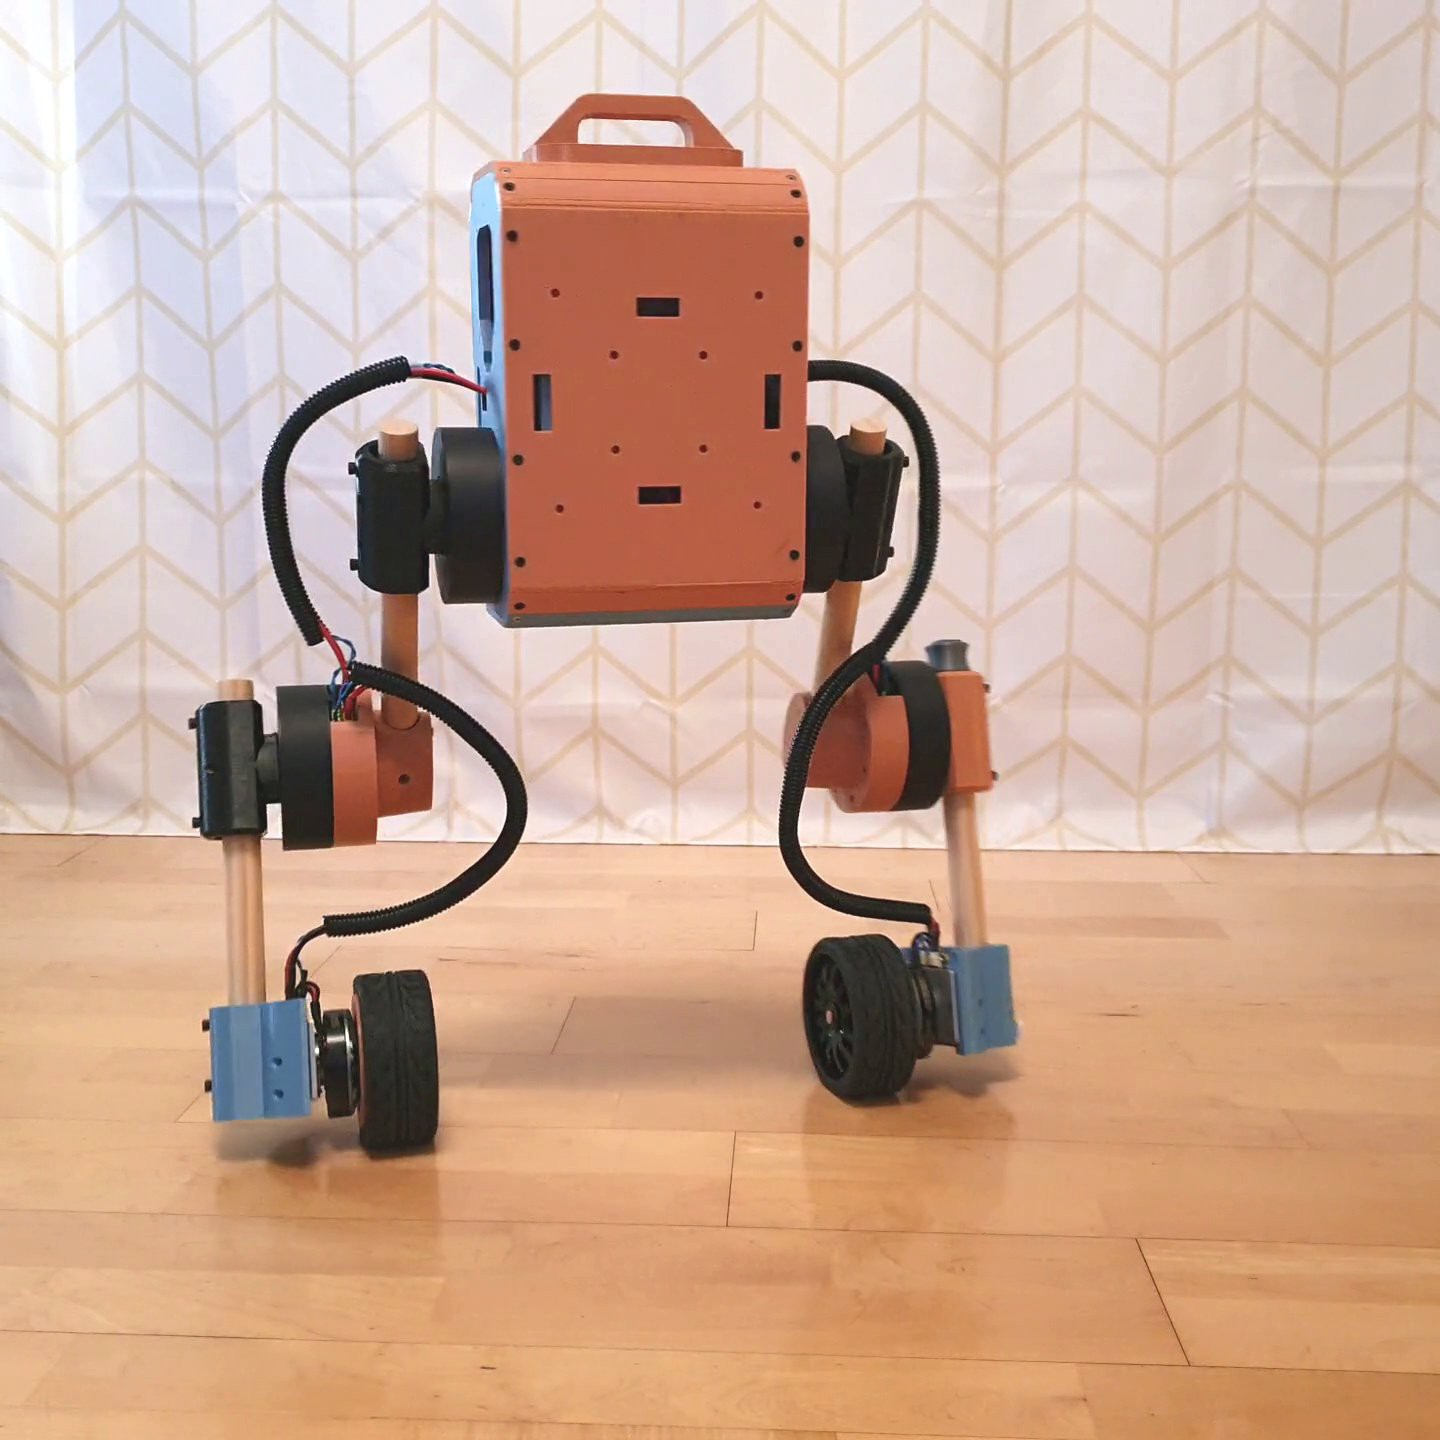
\includegraphics[height=2.5cm]{figures/upkie.jpg}
        \vspace{-3em}
    \end{figure}
\end{frame}

%%%%%%%%%%%%%%%%%%%%%%%%%%%%%%%%%%%%%%%%%%%%%%%%%%%%%%%%%%%%%%%%%%%%%%%%%%%%%%%%

\metroset{background=dark}
\section*{\textsc{Interlude 1: Robot descriptions}}
\metroset{background=light}

%%%%%%%%%%%%%%%%%%%%%%%%%%%%%%%%%%%%%%%%%%%%%%%%%%%%%%%%%%%%%%%%%%%%%%%%%%%%%%%%

\begin{frame}[fragile]{Robot descriptions}
    Load a robot description:
    \begin{minted}{python}
        from robot_descriptions.loaders.pinocchio import load_robot_description

        robot = load_robot_description("upkie_description")
    \end{minted}
    Visualize it:
    \begin{columns}
        \begin{column}{0.75\columnwidth}
            \begin{minted}{python}
                from pinocchio.visualize import MeshcatVisualizer

                robot.setVisualizer(MeshcatVisualizer())
                robot.initViewer(open=True)
                robot.loadViewerModel()
                robot.display(robot.q0)
            \end{minted}
        \end{column}
        \begin{column}{0.24\columnwidth}
            \begin{figure}
                \centering
                \includegraphics[width=\columnwidth]{figures/upkie_description.png}
            \end{figure}
        \end{column}
    \end{columns}
    \blfootnote{
        Setup: \mintinline{bash}{pip install meshcat pin robot_descriptions}
    }
\end{frame}

\begin{frame}[fragile]{Open source robot descriptions}
    Choose a description for the rest of this presentation:
    \begin{figure}
        \centering
        \includegraphics[width=0.9\columnwidth]{figures/robot-descriptions-social.png}
    \end{figure}
    \blfootnote{
        List: \url{https://github.com/robot-descriptions/robot_descriptions.py}
    }
\end{frame}

%%%%%%%%%%%%%%%%%%%%%%%%%%%%%%%%%%%%%%%%%%%%%%%%%%%%%%%%%%%%%%%%%%%%%%%%%%%%%%%%

\metroset{background=dark}
\section*{\textsc{Physics of walking}}
\metroset{background=light}

%%%%%%%%%%%%%%%%%%%%%%%%%%%%%%%%%%%%%%%%%%%%%%%%%%%%%%%%%%%%%%%%%%%%%%%%%%%%%%%%

\begin{frame}{Motivation}
    \begin{columns}
        \begin{column}{0.32\textwidth}
            \begin{figure}
                \centering
                \includegraphics[height=15em]{genfig/need-stabi-1.pdf}
            \end{figure}
            \begin{center}
                Plan$(t + \Delta t)$
            \end{center}
        \end{column}
        \begin{column}{0.33\textwidth}
            \begin{figure}
                \centering
                \includegraphics[height=15em]{genfig/need-stabi-2.pdf}
            \end{figure}
            \begin{center}
                Simulation$(t + \Delta t)$
            \end{center}
        \end{column}
        \begin{column}{0.32\textwidth}
            \begin{figure}
                \centering
                \includegraphics[height=15em]{genfig/need-stabi-3.pdf}
            \end{figure}
            \begin{center}
                Real$(t + \Delta t)$
            \end{center}
        \end{column}
    \end{columns}
\end{frame}

\begin{frame}{Honda P2}
    \begin{columns}
        \begin{column}{0.6\textwidth}
            Public demonstration in 1998:
            \begin{itemize}
                \item ``Zero'' Moment Point (ZMP) control
                \item Ground reaction force control
                \item Impact absorption:
            \end{itemize}
            \begin{figure}
                \centering
                \vspace{-0.5em}
                \includegraphics[height=7em]{figures/honda-rubber.png}
            \end{figure}
        \end{column}
        \begin{column}{0.4\textwidth}
            \centering
            \includegraphics[width=\textwidth]{figures/honda-p2.jpg}
        \end{column}
    \end{columns}
    \blfootcite{hirai1998icra}
\end{frame}

\begin{frame}{Physical model that makes it walk}
    \begin{columns}
        \begin{column}{0.5\textwidth}
            \begin{figure}
                \centering
                \includegraphics[height=4cm]{figures/honda-p2.jpg}
                \caption{Honda P2 walking}
            \end{figure}
        \end{column}
        \begin{column}{0.5\textwidth}
            \begin{figure}
                \centering
                \includegraphics[height=4cm]{genfig/linear-inverted-pendulum-flipped.pdf}
                \caption{Model it relies on}
            \end{figure}
        \end{column}
    \end{columns}
\end{frame}

\begin{frame}{Centroidal dynamics}
    \begin{columns}
        \begin{column}{0.49\textwidth}
            \begin{itemize}
                \item Whole-body dynamics: $$M \ddot{q} + N = S^T \tau + J^T f$$
                \item Actuated joints / floating base: 
                    \begin{align*}
                        M_a \ddot{q} + N_a & = \tau + J_a^T f \\
                        M_u \ddot{q} + N_u & = J_u^T f
                    \end{align*}
                \item Centroidal dynamics:
                    \begin{align*}
                        \ddot{c} & = g + \frac{1}{m} \sum_{i \in \mathsf{contacts}} f_i \\
                        \dot{L}_c & = \sum_{i \in \mathsf{contacts}} (p_i - c) \times f_i
                    \end{align*}
            \end{itemize}
        \end{column}
        \begin{column}{0.49\textwidth}
            \begin{figure}
                \centering
                \includegraphics[width=0.8\columnwidth]{genfig/centroidal-audren.pdf}
            \end{figure}
        \end{column}
    \end{columns}
    \blfootnote{
        Figure adapted from: \url{https://doi.org/10.1109/IROS.2014.6943129}
    }
\end{frame}

\begin{frame}{Center of pressure}
    \begin{figure}
        \centering
        \includegraphics[width=0.6\columnwidth]{genfig/cop-pressure-distrib.pdf}
        \caption{
            \textbf{(A)}~Continuous shearing/pressure distribution under a contact surface.
            \textbf{(B)}~Equivalent discrete force distribution, \emph{i.e.} producing the same wrench.
        }
    \end{figure}
    \blfootcite{caron2015icra}
\end{frame}

\begin{frame}{Zero-tilting Moment Point}
    \vspace{1em}
    \begin{columns}
        \begin{column}{0.6\textwidth}
            \begin{block}{Center of pressure (CoP)}
                Point $C$ on the contact surface where the resultant of
                \emph{pressure} forces $F^p$ is applied.
            \end{block}
            \begin{block}{Zero-tilting Moment Point (ZMP)}
                Point\emph{s} $Z$ where the moment of the contact wrench is
                aligned with the contact normal $n$.
            \end{block}
            \begin{itemize}
                \item Informally: the ZMP is the point where the net contact force is applied.
                \item Formally: the ZMP axis intersects the contact surface at the CoP.
            \end{itemize}
        \end{column}
        \begin{column}{0.4\textwidth}
            \centering
            \includegraphics[width=0.9\textwidth]{genfig/single-balance.pdf}
        \end{column}
    \end{columns}
    \blfootcite{sardain2004tsmc}
\end{frame}

\begin{frame}{Reduction to a point-mass model}
    \begin{columns}
        \begin{column}{0.5\textwidth}
            \begin{figure}
                \centering
                \includegraphics[height=4cm]{genfig/rigid-body-general.pdf}

                \caption{Net contact force does not go through CoM $c$ $\Rightarrow \dot{L}_c = I \ddot{\theta} > 0$, body rotates and translates.}
            \end{figure}
        \end{column}
        \begin{column}{0.5\textwidth}
            \begin{figure}
                \centering
                \includegraphics[height=4cm]{genfig/rigid-body-point-mass.pdf}
                \caption{Net contact force goes through CoM $c$ $\Rightarrow \dot{L}_c = 0$, body translates but does not rotate $\Rightarrow$ simpler!}
            \end{figure}
        \end{column}
    \end{columns}
    \begin{block}{Bottom line}
        A constant angular momentum reduces the system to translation
    \end{block}
\end{frame}

\begin{frame}{Linear inverted pendulum mode}
    \begin{columns}
        \begin{column}{0.55\textwidth}
            \textbf{Assumptions:}
            \begin{itemize}
                \item Rigid joints, sufficient power
                \item Conservation of angular momentum
                \item Constant CoM height
            \end{itemize}
            \begin{block}{Equation of motion}
                $$ \ddot{c} = \omega^2 (c - z) + g $$
            \end{block}
            \begin{itemize}
                \item $\omega$ is a constant
                \item $z$: \emph{zero-tilting moment point} (ZMP)
                \item In horiz. plane $+ g$ is usually omitted
            \end{itemize}
        \end{column}
        \begin{column}{0.45\textwidth}
            \begin{figure}
                \centering
                \includegraphics[width=\columnwidth]{genfig/linear-inverted-pendulum.pdf}
            \end{figure}
        \end{column}
    \end{columns}
    \blfootcite{kajita2001iros}
\end{frame}

\begin{frame}{Calculate the LIP constant}
    Recalling the physics and assumptions:
        \begin{itemize}
            \item Centroidal dynamics:
            \begin{align*}
                \ddot{c} & = g + \frac{1}{m} \sum_{i \in \mathsf{contacts}} f_i &
                \dot{L}_c & = \sum_{i \in \mathsf{contacts}} (p_i - c) \times f_i
            \end{align*}
            \item {Zero-tilting moment point}
                $$ \tau_z \times e_z = \left[\sum_{i \in \mathsf{contacts}} (p_i - z) \times f_i\right] \times e_z = 0 $$
            \item Constant height: $ c \cdot e_z = h $
            \item Angular momentum: $\dot{L}_c = 0$
        \end{itemize}
    \textbf{Question:} Can you derive the LIP equation $\ddot{c} = \omega^2 (c - z) + g$ from these equations, as well as the formula for $\omega$?
\end{frame}

\begin{frame}{ZMP support area}
    \begin{figure}
        \centering
        \includegraphics[height=5cm]{figures/zmp-infinite-friction.png}
        \caption{ZMP support area (large floor friction)}
    \end{figure}
\end{frame}

%%%%%%%%%%%%%%%%%%%%%%%%%%%%%%%%%%%%%%%%%%%%%%%%%%%%%%%%%%%%%%%%%%%%%%%%%%%%%%%%

\metroset{background=dark}
\section*{\textsc{Interlude 2: real-world controller}}
\metroset{background=light}

\metroset{background=dark}
\begin{frame}
    \begin{figure}
        \centering
        \includegraphics[width=5cm]{figures/airbus1.jpg}
        \caption{LIPM walking controller}
    \end{figure}
\end{frame}
\metroset{background=light}

%%%%%%%%%%%%%%%%%%%%%%%%%%%%%%%%%%%%%%%%%%%%%%%%%%%%%%%%%%%%%%%%%%%%%%%%%%%%%%%%

\begin{frame}[fragile]{LIPM walking controller}
    \begin{center}
        \includegraphics[height=4.5cm]{figures/lipm-walking-sim-standing.png}
    \end{center}
    \begin{minted}{bash}
        docker run -it --rm --user ayumi -e DISPLAY=${DISPLAY} \
            -v /tmp/.X11-unix:/tmp/.X11-unix:rw \
            stephanecaron/lipm_walking_controller \
            lipm_walking --floor
    \end{minted}
    \blfootnote{
        Source: \url{https://github.com/stephane-caron/lipm_walking_controller}
    }
\end{frame}

\begin{frame}[fragile]{Stair climbing}
    \begin{center}
        \includegraphics[height=4.5cm]{figures/lipm-walking-sim-stairs.png}
    \end{center}
    \begin{minted}{bash}
        docker run -it --rm --user ayumi -e DISPLAY=${DISPLAY} \
            -v /tmp/.X11-unix:/tmp/.X11-unix:rw \
            stephanecaron/lipm_walking_controller \
            lipm_walking --staircase
    \end{minted}
    \blfootnote{
        Source: \url{https://github.com/stephane-caron/lipm_walking_controller}
    }
\end{frame}
%%%%%%%%%%%%%%%%%%%%%%%%%%%%%%%%%%%%%%%%%%%%%%%%%%%%%%%%%%%%%%%%%%%%%%%%%%%%%%%%

\metroset{background=dark}
\section*{\textsc{Walking pattern generation}}
\metroset{background=light}

%%%%%%%%%%%%%%%%%%%%%%%%%%%%%%%%%%%%%%%%%%%%%%%%%%%%%%%%%%%%%%%%%%%%%%%%%%%%%%%%

\begin{frame}{Linear Model Predictive Control}
    \begin{columns}
        \begin{column}{0.6\textwidth}
            \begin{block}{Cost function}
                \begin{itemize}
                    \item Track desired ZMP reference
                    \item Track desired CoM velocity
                    \item Minimize CoM jerk
                \end{itemize}
            \end{block}
            \begin{block}{Constraints}
                \begin{itemize}
                    \item Consistency: equation of motion
                    \item Feasibility: ZMP in support area
                    \item Viability: terminal DCM
                \end{itemize}
            \end{block}
        \end{column}
        \begin{column}{0.4\textwidth}
            \begin{figure}
                \includegraphics[width=\columnwidth]{genfig/walkgen-com.pdf}
            \end{figure}
        \end{column}
    \end{columns}
    \blfootcite{wieber2006humanoids}
\end{frame}

\def\cd{\dot{c}}
\def\cdd{\ddot{c}}
\def\cddd{\dddot{{c}}}

\begin{frame}{Linear MPC is a Quadratic Program}
    \begin{align*}
        \min_{\cddd[1 \ldots N]} & 
            \quad w_z \sum_{k=1}^{N} \| p[k] - p^d[k] \|^2 + 
            w_v \sum_{k=1}^{N} \| \cd[k] - \cd^d[k] \|^2 +
            w_j \sum_{k=1}^{N} \| \cddd[k] \|^2 \\
        \mathsf{s.t.} \ \forall k
            & \quad c[k + 1] = {c}[k] + T \cd[k] + \frac{T^2}{2} \cdd[k] + \frac{T^3}{6} \cddd[k] \\
            & \quad \cd[k + 1] = \cd[k] + T \cdd[k] + \frac{T^2}{2} \cddd[k] \\
            & \quad \cdd[k + 1] = \cdd[k] + T \cddd[k] \\
            & \quad \textbf{Equation of motion:} \ \ p[k] = c[k] - \frac{\cdd[k]}{\omega^2} \\
            & \quad \textbf{Feasibility:} \ \ p_\mathsf{min}[k] \leq p[k] \leq p_\mathsf{max}[k] \\
            & \quad \textbf{Viability:} \ \ c[N] + \frac{\cd[N]}{\omega} = \xi^d[N] \\
    \end{align*}
    \vspace{-1em}
    \blfootcite{wieber2006humanoids}
\end{frame}

\begin{frame}[fragile]{Quadratic programming}
    Solve a quadratic program defined by:
    \[
        \begin{split}
        \begin{array}{ll}
            \underset{x}{\mbox{minimize}}
                & \frac{1}{2} x^T P x + q^T x \\
            \mbox{subject to}
                & G x \leq h \\
                & A x = b
        \end{array}
        \end{split}
    \]
    {Applications:} inverse kinematics, model predictive control, ...
    \begin{minted}{python}
        from qpsolvers import solve_qp

        M = np.array([[1., 2., 0.], [-8., 3., 2.], [0., 1., 1.]])
        P = M.T @ M  # this is a positive definite matrix
        q = np.array([3., 2., 3.]) @ M
        G = np.array([[1., 2., 1.], [2., 0., 1.], [-1., 2., -1.]])
        h = np.array([3., 2., -2.])
        x = solve_qp(P, q, G, h, solver="proxqp")
    \end{minted}
    \blfootnote{
        Setup: \mintinline{bash}{pip install proxsuite qpsolvers}
    }
\end{frame}

\begin{frame}{Lateral walking pattern}
    \begin{figure}
        \centering
        \includegraphics[height=6cm]{genfig/stairs-walkgen-lateral.pdf}
    \end{figure}
    \blfootnote{
        Explore real-robot data from the demo using \texttt{logs/display\_logs.py} in: \url{https://github.com/stephane-caron/lipm_walking_controller}
    }
\end{frame}

\begin{frame}{Lateral real robot}
    \begin{figure}
        \centering
        \includegraphics[height=6cm]{genfig/stairs-balancing-lateral.pdf}
    \end{figure}
\end{frame}

%%%%%%%%%%%%%%%%%%%%%%%%%%%%%%%%%%%%%%%%%%%%%%%%%%%%%%%%%%%%%%%%%%%%%%%%%%%%%%%%

\metroset{background=dark}
\section*{\textsc{Balance control}}
\metroset{background=light}

%%%%%%%%%%%%%%%%%%%%%%%%%%%%%%%%%%%%%%%%%%%%%%%%%%%%%%%%%%%%%%%%%%%%%%%%%%%%%%%%

\begin{frame}{Motivation}
    \begin{columns}
        \begin{column}{0.32\textwidth}
            \begin{figure}
                \centering
                \includegraphics[height=15em]{genfig/need-stabi-1.pdf}
            \end{figure}
            \begin{center}
                Plan$(t + \Delta t)$
            \end{center}
        \end{column}
        \begin{column}{0.33\textwidth}
            \begin{figure}
                \centering
                \includegraphics[height=15em]{genfig/need-stabi-2.pdf}
            \end{figure}
            \begin{center}
                Simulation$(t + \Delta t)$
            \end{center}
        \end{column}
        \begin{column}{0.32\textwidth}
            \begin{figure}
                \centering
                \includegraphics[height=15em]{genfig/need-stabi-3.pdf}
            \end{figure}
            \begin{center}
                Real$(t + \Delta t)$
            \end{center}
        \end{column}
    \end{columns}
\end{frame}

\begin{frame}{Linear inverted pendulum mode}
    \begin{columns}
        \begin{column}{0.55\textwidth}
            \textbf{Assumptions:}
            \begin{itemize}
                \item Rigid joints, sufficient power
                \item Conservation of angular momentum
                \item Constant CoM height
            \end{itemize}
            \begin{block}{Equation of motion}
                $$ \ddot{c} = \omega^2 (c - z) + g $$
            \end{block}
            \begin{itemize}
                \item $\omega$ is a constant
                \item $z$: \emph{zero-tilting moment point} (ZMP)
                \item In horiz. plane $+ g$ is usually omitted
            \end{itemize}
        \end{column}
        \begin{column}{0.45\textwidth}
            \begin{figure}
                \centering
                \includegraphics[width=\columnwidth]{genfig/linear-inverted-pendulum.pdf}
            \end{figure}
        \end{column}
    \end{columns}
    \blfootcite{kajita2001iros}
\end{frame}

\begin{frame}{Divergent component of motion}
    \begin{columns}
        \begin{column}{0.55\textwidth}
            \begin{itemize}
                \item Linear inverted pendulum mode: $\cdd = \omega^2 (c - p)$
                \item Divergent component of motion: $\xi := c + \frac{\cd}{\omega}$
            \end{itemize}
            \begin{block}{Equation of motion}
                $$ \xid = \omega (\xi - p) $$
            \end{block}
            \begin{itemize}
                \item Point $\xi_g$ where to step instantaneously to stop walking
            \end{itemize}
        \end{column}
        \begin{column}{0.45\textwidth}
            \begin{figure}
                \centering
                \includegraphics[width=\columnwidth]{genfig/lip-with-dcm.pdf}
            \end{figure}
        \end{column}
    \end{columns}
\end{frame}

\begin{frame}{Balance control with feet}
    \begin{columns}
        \begin{column}{0.55\columnwidth}
            \begin{itemize}
                \item DCM dynamics:
                    $$ \xid = \omega (\xi - z) $$
                \item Regulate the ZMP by \textbf{force control}:
                    $$ z = z^d + \xi - k(\xi^d - \xi)$$
                \item Closed loop: $\xi \to \xi^d$
                    $$ \xid = k\omega (\xi^d - \xi) $$
                \item As long as the ZMP target is feasible...
            \end{itemize}
        \end{column}
        \begin{column}{0.45\columnwidth}
            \begin{figure}
                \centering
                \includegraphics[width=0.7\columnwidth]{genfig/balance-feet.pdf}
            \end{figure}
        \end{column}
    \end{columns}
\end{frame}

\begin{frame}{Balance control with wheels}
    \begin{columns}
        \begin{column}{0.55\columnwidth}
            \begin{itemize}
                \item DCM dynamics:
                    $$ \xid = \omega (\xi - z) $$
                \item Regulate the ZMP by \textbf{velocity control}:
                    $$ z = z^d + \xi - k(\xi^d - \xi)$$
                \item Closed loop: $\xi \to \xi^d$
                    $$ \xid = k\omega (\xi^d - \xi) $$
                \item As long as the ZMP target is feasible...
            \end{itemize}
        \end{column}
        \begin{column}{0.45\columnwidth}
            \begin{figure}
                \centering
                \includegraphics[width=0.7\columnwidth]{genfig/balance-wheel.pdf}
            \end{figure}
        \end{column}
    \end{columns}
\end{frame}

%%%%%%%%%%%%%%%%%%%%%%%%%%%%%%%%%%%%%%%%%%%%%%%%%%%%%%%%%%%%%%%%%%%%%%%%%%%%%%%%

\metroset{background=dark}
\section*{\textsc{Interlude 3: Wheeled biped}}
\metroset{background=light}

\metroset{background=dark}
\begin{frame}
    \begin{figure}
        \centering
        \includegraphics[width=5cm]{figures/upkie_locomotion.jpg}
        \caption{Pink controller}
    \end{figure}
\end{frame}
\metroset{background=light}

\begin{frame}[fragile]{Upkie locomotion}
    The locomotion software for Upkie comes batteries included:
    \begin{minted}{bash}
        git clone https://github.com/tasts-robots/upkie_locomotion.git
        cd upkie_locomotion
        ./tools/bazelisk run -c opt //agents/blue_balancer:bullet
    \end{minted}
    Bazel will download and build everything (no installation required).

    \textbf{Extend it!} Make it move the wheels back and forth while balancing.

    \begin{figure}
        \centering
        \includegraphics[width=\columnwidth]{figures/upkie_locomotion_bullet.png}
    \end{figure}
    \blfootnote{
        Repository: \url{https://github.com/tasts-robots/upkie_locomotion}
    }
\end{frame}

%%%%%%%%%%%%%%%%%%%%%%%%%%%%%%%%%%%%%%%%%%%%%%%%%%%%%%%%%%%%%%%%%%%%%%%%%%%%%%%%

\metroset{background=dark}
\section*{\textsc{What did we see?}}
\metroset{background=light}

%%%%%%%%%%%%%%%%%%%%%%%%%%%%%%%%%%%%%%%%%%%%%%%%%%%%%%%%%%%%%%%%%%%%%%%%%%%%%%%%

\begin{frame}{What did we see?}
    From INFO to ROB:
    \begin{itemize}
        \item One possible use of one's \emph{engagement d\'{e}cennal}
    \end{itemize}
    Balancing legged robots:
    \begin{itemize}
        \item \textbf{Physics:} linear inverted pendulum, ZMP, support area
        \item \textbf{Trajectory generation:} ideal trajectory
        \item \textbf{Balance control:} adjust ZMP based on the CoM/DCM
    \end{itemize}
    Applies to humanoids, wheeled bipeds, flywheeled coffee makers, etc.
    \blfootnote{
        Questions? $\to$ \url{mailto:stephane.caron@normalesup.org}
    }
\end{frame}

\begin{frame}{That's all folks!}
    \vspace{2em}
    \begin{figure}
        \centering
        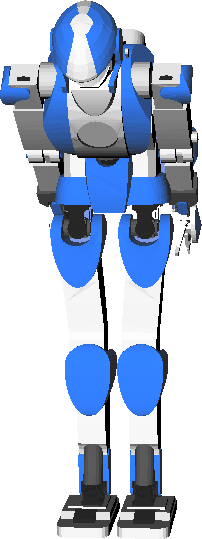
\includegraphics[height=10em]{genfig/thanks.pdf}
    \end{figure}
\end{frame}

%%%%%%%%%%%%%%%%%%%%%%%%%%%%%%%%%%%%%%%%%%%%%%%%%%%%%%%%%%%%%%%%%%%%%%%%%%%%%%%%

\metroset{background=dark}
\section*{\textsc{Bibliography}}
\metroset{background=light}

%%%%%%%%%%%%%%%%%%%%%%%%%%%%%%%%%%%%%%%%%%%%%%%%%%%%%%%%%%%%%%%%%%%%%%%%%%%%%%%%

\renewcommand*{\bibfont}{\footnotesize}
\setbeamertemplate{bibliography item}{\insertbiblabel}

\begin{frame}[allowframebreaks]{References}
    \printbibliography[heading=none]
\end{frame}

%%%%%%%%%%%%%%%%%%%%%%%%%%%%%%%%%%%%%%%%%%%%%%%%%%%%%%%%%%%%%%%%%%%%%%%%%%%%%%%%

\metroset{background=dark}
\section*{\textsc{Bonus slides: inverse kinematics}}
\metroset{background=light}

%%%%%%%%%%%%%%%%%%%%%%%%%%%%%%%%%%%%%%%%%%%%%%%%%%%%%%%%%%%%%%%%%%%%%%%%%%%%%%%%

\begin{frame}[fragile]{Task-based inverse kinematics}
    Define a task for each foot:
    \begin{minted}{python}
        from pink.tasks import BodyTask

        tasks = [
            BodyTask(f"{leg}_contact", position_cost=1., orientation_cost=1.)
            for leg in ("left", "right")  # adapt to the robot you picked
        ]
    \end{minted}
    Initialize task targets:
    \begin{minted}{python}
        from pink import apply_configuration

        configuration = apply_configuration(robot, robot.q0)
        for task in tasks:
            task.set_target_from_configuration(configuration)
    \end{minted}
    \blfootnote{
        Setup: \mintinline{bash}{pip install pin-pink}
    }
\end{frame}

\begin{frame}[fragile]{Target scenario}
    Let's display our targets for convenience:
    \begin{minted}{python}
        import meshcat_shapes

        for task in tasks:
            meshcat_shapes.frame(robot.viewer[f"{task.body}_target"])
    \end{minted}
    And define the trajectory of our task targets:
    \begin{columns}
        \begin{column}{0.75\columnwidth}
            \begin{minted}{python}
                def update_targets(tasks, t, dt):
                    for task in tasks:
                        u = 0.2 * np.array([2.0, 0.0, 1.0])
                        T = task.transform_target_to_world
                        T.translation += np.sin(2 * t) * u * dt

                        frame = robot.viewer[f"{task.body}_target"]
                        frame.set_transform(T.np)
            \end{minted}
        \end{column}
        \begin{column}{0.24\columnwidth}
            \begin{figure}
                \centering
                \includegraphics[width=\columnwidth]{genfig/task-targets.pdf}
            \end{figure}
        \end{column}
    \end{columns}
    \blfootnote{
        Setup: \mintinline{bash}{pip install meshcat_shapes}
    }
\end{frame}

\begin{frame}[fragile]{Closed-loop inverse kinematics}
    \begin{columns}
        \begin{column}{0.75\columnwidth}
            \begin{minted}{python}
                from pink import solve_ik
                from loop_rate_limiters import RateLimiter

                rate = RateLimiter(frequency=200)
                dt = rate.period
                for t in np.arange(0., 5., dt):
                    update_targets(tasks, t, dt)
                    velocity = solve_ik(
                        configuration, tasks, dt, solver="proxqp"
                    )
                    q = configuration.integrate(velocity, dt)
                    configuration = apply_configuration(robot, q)
                    robot.display(q)
                    rate.sleep()
            \end{minted}
            Behavior when tasks become unfeasible?
        \end{column}
        \begin{column}{0.24\columnwidth}
            \begin{figure}
                \centering
                \includegraphics[width=\columnwidth]{figures/upkie-ik.png}
            \end{figure}
        \end{column}
    \end{columns}
    \blfootnote{
        Setup: \mintinline{bash}{pip install loop-rate-limiters proxsuite pin-pink}
    }
\end{frame}

%%%%%%%%%%%%%%%%%%%%%%%%%%%%%%%%%%%%%%%%%%%%%%%%%%%%%%%%%%%%%%%%%%%%%%%%%%%%%%%%

\end{document}
